\documentclass[twoside,12pt]{article}

% This format is based on that of the Journal of Machine Learning Research,
% with some structural changes to encourage readability by practitioners
%
% Any additional packages needed should be included after jemlp.
% Note that jemlp.sty includes epsfig, amssymb, biblatex, graphicx,
% and hyperref, and defines many common macros, such as 'proof' 
% and 'example'.
%
% This style sheet replaces the long-form end-of-manuscript bibliography
% with footnote citations, using \citef{}, one citation at a time. This
% should help to both keep long citations from clogging up the actual text,
% while also informing readers as to the full title and authors of the paper
% referenced without needing to go to the end of the manuscript.

\usepackage{jemlp}

% Definitions of handy macros can go here

\newcommand{\dataset}{{\mathcal D}}
\newcommand{\fracpartial}[2]{\frac{\partial #1}{\partial  #2}}

% Heading arguments are {volume}{year}{submitted}{published}{author-full-names}

\jemlpheading{1}{2022}{1/22}{2/22}{Jonathan S. Kent and Jonathan S. Kent}

% Short headings should be running head and authors last names

\ShortHeadings{JEMLP Manuscript Format}{Kent et al}
\firstpageno{1}

\begin{document}

\title{Journal of Efficient Machine Learning Practice\\ Manuscript Format}

\author{\name Jonathan S. Kent \email jonathan.s.kent@lmco.com \\
       \addr Advanced Technology Center\\
       Lockheed Martin\\
       Sunnyvale, CA 94089, USA
       \AND
       \name Jonathan S. Kent \email jskent2@illinois.edu \\
       \addr Department of Mathematics\\
       University of Illinois at Urbana-Champaign\\
       Urbana, IL 61081, USA}

\editor{Jonathan S. Kent}

\maketitle

\begin{abstract}
Welcome to the Journal of Efficient Machine Learning Practice. This is a journal that will be focusing on efficiency, robustness, and real-world application of Machine Learning, and also to promote the writing of reader-friendly articles. If that seems up your alley, you are welcome to make an account and submit a paper to the \href{https:\\www.jemlp.org}{Journal of Efficient Machine Learning Practice}.

The purpose of the abstract is unchanged. Briefly explain the context, core problems, methodology, and results of your paper.
\end{abstract}

\begin{keywords}
  Manuscript, Format
\end{keywords}

\begin{readnote}
For the note to readers, please write a very brief explanation of the real-world impacts of your paper in plain language, such as examples of problems it could help solve. Also, list any nonstandard prerequisites for understanding your work, anything beyond typical undergraduate education in Science, Mathematics, or Engineering, additionally assuming a general background in Machine and Deep Learning. If your paper relies on, say, Differential Calculus, you can assume your readers are already familiar, but please make a note if you're using results from Differential Geometry. You may assume your readers are familiar with, for example, Neural Networks and the Adam optimization algorithm, but please list any recent or lesser-known papers if your work cannot be understood without reading them first.
\end{readnote}



\section{Introduction}

Please exercise a reasonable level of authorial judgement when formatting your manuscript. Rather than prescribe specific packages or designs that must be used for figures, tables, algorithms in psuedocode, or Mathematical formulae, you are encouraged to go with whatever you feel best communicates your ideas and results. Citations will be given as footnotes, like so\cite{einstein1905electrodynamics}, and if you wish to refer to the work being cited in text, you may do so by writing a reference to the work, e.g. In \textit{the Muqaddimah}\cite{khaldun2015muqaddimah}, Ibn Khaldun characterizes societies based on the strength of their ``group feeling." Multiple citations at the same time will produce one combined entry in the footnotes.

Your prose, typography, and notation should be clear and explanatory, and be neither too dense to easily communicate its ideas, nor too long in getting to its main arguments. You should explain what you're doing, why you're doing it, and by what mechanism you're achieving it. Someone who is not a deep expert in your particular subfield should be able to follow your train of thought through your writing, and gain expertise. Otherwise, there are no page minimums or maximums to be concerned about.

Additionally, you may reference sections from the IPython/Jupyter notebook that will be paired with your manuscript. But please try not to do this excessively, to help with the flow of reading your work.

\section{Figures}

\begin{figure}
    \centering
    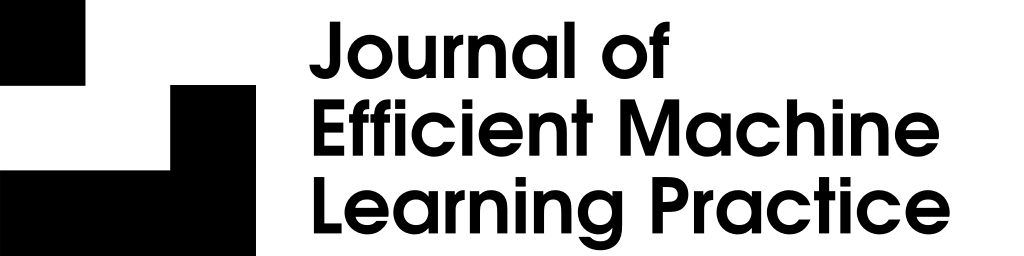
\includegraphics[width=0.5\textwidth]{example_figure}
    \caption{An example of a scientific graphic or figure}
    \label{fig:my_label}
\end{figure}

\begin{table}
    \centering
    \begin{tabular}{c|cc}
        A & B & C \\
        \hline
        a & b & c \\ 
        d & e & f \\
    \end{tabular}
    \caption{An example of a table containing results. Please use your own judgement to format tables such as to be clear and easy to read, without too many unnecessary lines.}
    \label{tab:my_table}
\end{table}

Figures and tables should appear at the top of the page, as close to the text referencing them as possible.



% Acknowledgements should go at the end, before the appendices

\acks{Setting up this journal has been made possible by support from the Lockheed Martin Advanced Technology Center.}

\appendix
\section*{Appendix A.}
\label{app:theorem}

Appendices should be reserved for large tables of numerical results, Mathematical proofs, and graphical figures that are ancillary to the over-all thrust of the manuscript. If they are needed to understand your work, they should be included in or near the section where they appear. Please note that the typefaces for text and for Mathematics differ, such that numbers, e.g. 0123456789 and $0123456789$, appear visually distinct. If a number is used in a Mathematical context, but placed in text, typeset it as Mathematics.

The following example appendix was drawn from the template paper for the Journal of Machine Learning Research\cite{meila2000learning}, upon which this format was based.\\
% Note: in this sample, the section number is hard-coded in. Following
% proper LaTeX conventions, it should properly be coded as a reference:

%In this appendix we prove the following theorem from
%Section~\ref{sec:textree-generalization}:

In this appendix we prove the following theorem from
Section~6.2:

\noindent
{\bf Theorem} {\it Let $u,v,w$ be discrete variables such that $v, w$ do
not co-occur with $u$ (i.e., $u\neq0\;\Rightarrow \;v=w=0$ in a given
dataset $\dataset$). Let $N_{v0},N_{w0}$ be the number of data points for
which $v=0, w=0$ respectively, and let $I_{uv},I_{uw}$ be the
respective empirical mutual information values based on the sample
$\dataset$. Then
\[
	N_{v0} \;>\; N_{w0}\;\;\Rightarrow\;\;I_{uv} \;\leq\;I_{uw}
\]
with equality only if $u$ is identically $0$.} \hfill\BlackBox

\noindent
{\bf Proof}. We use the notation:
\[
P_v(i) \;=\;\frac{N_v^i}{N},\;\;\;i \neq 0;\;\;\;
P_{v0}\;\equiv\;P_v(0)\; = \;1 - \sum_{i\neq 0}P_v(i).
\]
These values represent the (empirical) probabilities of $v$
taking value $i\neq 0$ and 0 respectively.  Entropies will be denoted
by $H$. We aim to show that $\fracpartial{I_{uv}}{P_{v0}} < 0$....\\

\end{document}